\chapter{Trabalhos Relacionados}\label{trab_rela}


\section{Competências requeridas pela avaliação de redação do enem}

De acordo com ~\cite{silvio_taynan:2017} a prova de redação do ENEM é avaliada levando em conta uma matriz de referência listada na Tabela ~\ref{tab:matriz_referencia}. Essa matriz, desenvolvida pelo ~\cite{edital_enem:2016}, com a colaboração de especialistas, foi elaborada com o objetivo de operacionalizar o exame. A matriz apresenta cinco competências, para cada competência expressa para redação existem níveis de conhecimento associados de 0 a 5.

De acordo com ~\cite{braga:2015}, no texto de redação, o candidato defenderá uma opinião a respeito do tema proposto, de forma coerente e coesa, embasado em argumentos consistentes. O texto será redigido respeitando a escrita formal da Língua Portuguesa. Ao fim, o candidato elabora uma proposta de intervenção social para o problema apresentado no desenvolvimento do texto que respeite os direitos humanos.

\begin{longtable}{|c|l|l|}
    \caption{Matriz de referência elaborada pelo INEP.}
    \label{tab:matriz_referencia}
    \endfirsthead
    \multicolumn{3}{l}%
    {Tabela \thetable{} (continuação)}
    \endhead
    \multicolumn{3}{l}%
    {Continua na próxima página}\\
    \endfoot
    \endlastfoot
    \hline
    \multirow{7}{*}{\textbf{I}} & \multicolumn{2}{l|}{\textbf{Demonstrar domínio da norma padrão da língua escrita.}} \\ \cline{2-3} 
     & 0 & \begin{tabular}[c]{@{}l@{}}Demonstra desconhecimento da modalidade escrita formal da \\ língua portuguesa.\end{tabular} \\ \cline{2-3} 
     & 1 & \begin{tabular}[c]{@{}l@{}}Demonstra domínio precário da modalidade escrita formal da \\ língua por-tuguesa, de forma sistemática, com diversificados e \\ frequentes desvios gramaticais, de escolha de registro e de \\ convenções da escrita.\end{tabular} \\ \cline{2-3} 
     & 2 & \begin{tabular}[c]{@{}l@{}}Demonstra domínio insuficiente da modalidade escrita formal \\ da língua portuguesa, com muitos desvios gramaticais, de \\ escolha de registro e de convenções da escrita.\end{tabular} \\ \cline{2-3} 
     & 3 & \begin{tabular}[c]{@{}l@{}}Demonstra domínio mediano da modalidade escrita formal da \\ língua portuguesa e de escolha de registro, com alguns desvios \\ gramaticais e de convenções da escrita.\end{tabular} \\ \cline{2-3} 
     & 4 & \begin{tabular}[c]{@{}l@{}}Demonstra bom domínio da modalidade escrita formal da língua \\ portuguesa e de escolha de registro,com poucos desvios \\ gramaticais e de convenções da escrita.\end{tabular} \\ \cline{2-3} 
     & 5 & \begin{tabular}[c]{@{}l@{}}Demonstra excelente domínio da modalidade escrita formal da \\ língua portuguesa e de escolha deregistro. Desvios gramaticais \\ ou de convenções da escrita serão aceitos somente como \\ excepcionalidade equando não caracterizem reincidência.\end{tabular} \\ \hline
    \multirow{7}{*}{\textbf{II}} & \multicolumn{2}{l|}{\textbf{\begin{tabular}[c]{@{}l@{}}Compreender a proposta de redação e aplicar conceitos \\ das varias áreas de conhecimento paradesenvolver o tema, \\ dentro dos limites estruturais do texto \\ dissertativo-argumentativo em prosa.\end{tabular}}} \\ \cline{2-3} 
     & 0 & \begin{tabular}[c]{@{}l@{}}``Fuga ao tema/não atendimento à estrutura \\ dissertativo-argumentativa''.\end{tabular} \\ \cline{2-3} 
     & 1 & \begin{tabular}[c]{@{}l@{}}Apresenta o assunto, tangenciando o tema ou demonstra \\ domínio precário do texto dissertativo-argumentativo, com \\ traços constantes de outros tipos textuais\end{tabular} \\ \cline{2-3} 
     & 2 & \begin{tabular}[c]{@{}l@{}}Desenvolve o tema recorrendo à cópia de trechos dos textos \\ motivadores ou apresenta domínioinsuficiente do texto \\ dissertativo-argumentativo, não atendendo à estrutura com \\ proposição, argumentação econclusão.\end{tabular} \\ \cline{2-3} 
     & 3 & \begin{tabular}[c]{@{}l@{}}Desenvolve o tema por meio de argumentação previsível e \\ apresenta domínio mediano do textodissertativo-argumentativo, \\ com proposição, argumentação e conclusão.\end{tabular} \\ \cline{2-3} 
     & 4 & \begin{tabular}[c]{@{}l@{}}Desenvolve o tema por meio de argumentação consistente e \\ apresenta bom domínio do textodissertativo-argumentativo, \\ com proposição, argumentação e conclusão.\end{tabular} \\ \cline{2-3} 
     & 5 & \begin{tabular}[c]{@{}l@{}}Desenvolve o tema por meio de argumentação consistente, a \\ partir de um repertório socioculturalprodutivo e apresenta \\ excelente domínio do texto dissertativo-argumentativo.\end{tabular} \\ \hline
    \multirow{7}{*}{\textbf{III}} & \multicolumn{2}{l|}{\textbf{\begin{tabular}[c]{@{}l@{}}Selecionar, relacionar, organizar e interpretar informações, \\ fatos, opiniões e argumentos em defesa de umponto de vista.\end{tabular}}} \\ \cline{2-3} 
     & 0 & \begin{tabular}[c]{@{}l@{}}Apresenta informações, fatos e opiniões não relacionados \\ ao tema e sem defesa de um ponto devista.\end{tabular} \\ \cline{2-3} 
     & 1 & \begin{tabular}[c]{@{}l@{}}Apresenta informações, fatos e opiniões pouco relacionados \\ ao tema ou incoerentes e sem defesa deum ponto de vista.\end{tabular} \\ \cline{2-3} 
     & 2 & \begin{tabular}[c]{@{}l@{}}Apresenta informações, fatos e opiniões relacionados ao \\ tema, mas desorganizados ou contraditóriose limitados aos \\ argumentos dos textos motivadores, em defesa de um \\ ponto de vista.\end{tabular} \\ \cline{2-3} 
     & 3 & \begin{tabular}[c]{@{}l@{}}Apresenta informações, fatos e opiniões relacionados ao tema, \\ limitados aos argumentos dos textosmotivadores e pouco \\ organizados, em defesa de um ponto de vista.\end{tabular} \\ \cline{2-3} 
     & 4 & \begin{tabular}[c]{@{}l@{}}Apresenta informações, fatos e opiniões relacionados ao tema, \\ de forma organizada, com indícios deautoria, em defesa de \\ um ponto de vista.\end{tabular} \\ \cline{2-3} 
     & 5 & \begin{tabular}[c]{@{}l@{}}Apresenta informações, fatos e opiniões relacionados ao \\ tema proposto, de forma consistente e organizada, configurando \\ autoria, em defesa de um ponto de vista.\end{tabular} \\ \hline
    \multirow{7}{*}{\textbf{IV}} & \multicolumn{2}{l|}{\textbf{\begin{tabular}[c]{@{}l@{}}Demonstrar conhecimento dos mecanismos linguísticos \\ necessários para a construção da argumentação.\end{tabular}}} \\ \cline{2-3} 
     & 0 & Não articula as informações. \\ \cline{2-3} 
     & 1 & Articula as partes do texto de forma precária. \\ \cline{2-3} 
     & 2 & \begin{tabular}[c]{@{}l@{}}Articula as partes do texto, de forma insuficiente, com muitas \\ inadequações e apresenta repertóriolimitado de recursos coesivos.\end{tabular} \\ \cline{2-3} 
     & 3 & \begin{tabular}[c]{@{}l@{}}Articula as partes do texto, de forma mediana, com inadequações, \\ e apresenta repertório poucodiversificado de recursos coesivos.\end{tabular} \\ \cline{2-3} 
     & 4 & \begin{tabular}[c]{@{}l@{}}Articula as partes do texto com poucas inadequações e apresenta \\ repertório diversificado de recursoscoesivos.\end{tabular} \\ \cline{2-3} 
     & 5 & \begin{tabular}[c]{@{}l@{}}Articula bem as partes do texto e apresenta repertório diversificado \\ de recursos coesivos.\end{tabular} \\ \hline
    \multirow{7}{*}{\textbf{V}} & \multicolumn{2}{l|}{\textbf{\begin{tabular}[c]{@{}l@{}}Elaborar proposta de intervenção para o problema abordado, \\ respeitando os direitos humanos.\end{tabular}}} \\ \cline{2-3} 
     & 0 & \begin{tabular}[c]{@{}l@{}}Não apresenta proposta de intervenção ou apresenta proposta não \\ relacionada ao tema ou ao assunto.\end{tabular} \\ \cline{2-3} 
     & 1 & \begin{tabular}[c]{@{}l@{}}Apresenta proposta de intervenção vaga, precária ou relacionada \\ apenas ao assunto.\end{tabular} \\ \cline{2-3} 
     & 2 & \begin{tabular}[c]{@{}l@{}}Elabora, de forma insuficiente, proposta de intervenção relacionada \\ ao tema, ou não articulada com adiscussão desenvolvida no texto.\end{tabular} \\ \cline{2-3} 
     & 3 & \begin{tabular}[c]{@{}l@{}}Elabora, de forma mediana, proposta de intervenção relacionada ao \\ tema e articulada à discussãodesenvolvida no texto.\end{tabular} \\ \cline{2-3} 
     & 4 & \begin{tabular}[c]{@{}l@{}}Elabora bem proposta de intervenção relacionada ao tema e \\ articulada à discussão desenvolvida notexto.\end{tabular} \\ \cline{2-3} 
     & 5 & \begin{tabular}[c]{@{}l@{}}Elabora muito bem proposta de intervenção, detalhada, relacionada \\ ao tema e articulada à discussãodesenvolvida no texto.\end{tabular} \\ \hline
\end{longtable}

% 2) classificadores de textos
\section{Modelo de representação de texto mais adequado à classificação}

Segundo ~\cite{alexandra_alves:2010} o BOW (\textit{Bag of Words}) é o modelo mais utilizado em aplicações de classificação de texto. Com baixo custo em termos de processamento este modelo transforma a cadeia de caracteres de um documento num conjunto de palavras, registrando além da presença de uma palavra, a sua frequência.

Entretanto propriedades básicas do texto, como a ordem em que as palavras ocorrem e a pontuação, são ignoradas, além da incapacidade em capturar a semântica do texto, isto é, há palavras com significados distintos que apesar de serem exatamente iguais têm significados diferentes, dependendo do contexto em que são utilizadas.

Obviamente, termos que aparecem em todos os documentos não serão analisados, geralmente são os pronomes, artigos e as preposições. Estes termos são chamados de \textit{stop words}, não são úteis dado que têm uma semântica fraca e somente desempenham um papel funcional no texto. Para melhorar os métodos de processamento normalmente são removidas, em vários casos a remoção das \textit{stop words} não traz consequências graves.

Na Tabela ~\ref{tab:bow}, \textbf{w}\textsubscript{i} representa uma palavra, \textbf{d}\textsubscript{j} representa um documento e \textbf{p}\textsubscript{ij} o peso atribuído a cada palavra no documento.

\begin{longtable}{|c|c|c|c|c|c|}
    \caption{Modelo \textit{Bag of Words}}
    \label{tab:bow}
    \endfirsthead
    \multicolumn{6}{l}%
    {Tabela \thetable{} (continuação)}
    \endhead
    \multicolumn{6}{l}%
    {Continua na próxima página}\\
    \endfoot
    \endlastfoot
    \hline  & \textbf{w}\textsubscript{1} & \textbf{w}\textsubscript{2} & \textbf{w}\textsubscript{3} & \textbf{w}\textsubscript{...} & \textbf{w}\textsubscript{n} \\
    \hline \textbf{d}\textsubscript{1} & p\textsubscript{11} & p\textsubscript{12} & p\textsubscript{13} & p\textsubscript{...} & p\textsubscript{1n} \\
    \hline \textbf{d}\textsubscript{2} & p\textsubscript{21} & p\textsubscript{22} & p\textsubscript{23} & p\textsubscript{...} & p\textsubscript{2n} \\
    \hline \textbf{d}\textsubscript{3} & p\textsubscript{31} & p\textsubscript{32} & p\textsubscript{33} & p\textsubscript{...} & p\textsubscript{3n} \\
    \hline \textbf{d}\textsubscript{4} & p\textsubscript{41} & p\textsubscript{42} & p\textsubscript{43} & p\textsubscript{...} & p\textsubscript{4n} \\
    \hline \textbf{d}\textsubscript{n} & p\textsubscript{n1} & p\textsubscript{n2} & p\textsubscript{n3} & p\textsubscript{...} & p\textsubscript{nn} \\
    \hline
\end{longtable}

Ainda segundo ~\cite{alexandra_alves:2010} existem várias medidas para calcular os valores dos pesos de p\textsubscript{ij}. Essas medidas podem ser classificadas em dois tipos distintos: baseadas em frequências e binárias. Os pesos baseados em frequência visam contabilizar o número de ocorrências de um dado termo num determinado documento, servindo como base para diversas medidas estatísticas e os pesos binários indicam a ocorrência ou não de um dado termo num determinado documento.

\section{Aprendizado de máquina}

Segundo ~\cite{monard_baranauskas:2003} ``A indução é a forma de inferência lógica que permite obter conclusões genéricas sobre um conjunto particular de exemplos.'' Na indução, um conceito é aprendido efetuando-se inferência indutiva sobre os exemplos apresentados. O aprendizado indutivo pode ser dividido em supervisionado e não-supervisionado como ilustrado na Figura ~\ref{fig:aprendizado_indutivo}.  

No aprendizado não-supervisionado, o algoritmo de aprendizado analisa os exemplos fornecidos e tenta determinar se alguns deles podem ser agrupados de alguma maneira, formando clusters ou agrupamentos. Já no aprendizado supervisionado é fornecido ao algoritmo de aprendizado um conjunto de exemplos de treinamento para os quais o rótulo da classe associada é conhecido.

\begin{figure}[H]
\begin{center}
    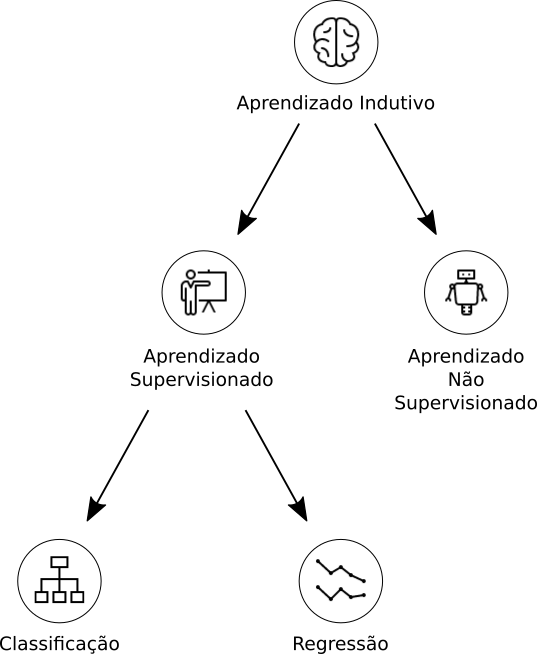
\includegraphics[scale=0.75]{figuras/aprendizado_indutivo.png}
\end{center}
\caption{A hierarquia do aprendizado indutivo}
\label{fig:aprendizado_indutivo}
\end{figure}

De acordo com ~\cite{porthos_motta:2016} classificadores são utilizados para a predição de classes de objetos e pode ser dita como o processo de generalização dos dados a partir de diferentes instâncias. Existe uma tendência de se referir a problemas com uma resposta quantitativas como problemas de regressão e aqueles com uma resposta qualitativa como problemas de classificação.

Dado um conjunto de exemplos como ilustrado na Figura ~\ref{fig:processo_classificacao}, os classificadores devem encontrar uma função geral capaz de prever adequadamente as saídas para novos exemplos, após o treinamento, o classificador é avaliado e se necessário o processo de classificação pode ser ajustado usando o conhecimento sobre o domínio do problema para escolher os dados de entrada ao algoritmo de aprendizado. 

% processo de classificação

\begin{figure}[H]
\begin{center}
    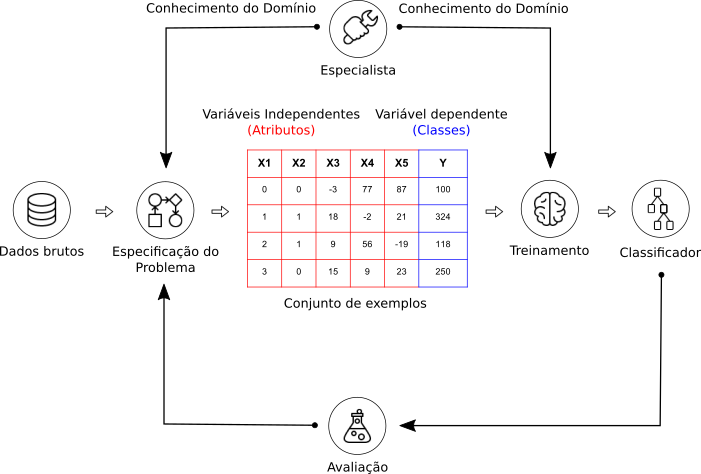
\includegraphics[scale=0.75]{figuras/processo_classificacao.png}
\end{center}
\caption{Processo de Classificação}
\label{fig:processo_classificacao}
\end{figure}

% 4) Orange mineração de dados

\section{Ferramenta para mineração de dados}

Diversas ferramentas disponíveis para exploração de dados dispõem de soluções para o processamento e a análise das informações de forma agil e simples. Em uma analise comparativa ~\cite{boscarioli2014avaliaccao} demonstra que não existe uma única ferramenta com caracteristicas melhores para todas as aplicações em mineração de dados.

Em um estudo que comparou quatro ferramentas (KMINE, \textit{Orange}, Tanagra, Weka), todas de código aberto, gratuitas e muito utilizadas na pesquisa e na academia, ~\cite{wahbeh2011comparison} concluiu que a ferramenta Weka apresentou o melhor desempenho, seguido pelo \textit{Orange}, e, depois, pelo KMINE e Tanagra.

Para este trabalho, foi escolhida a ferramenta \textit{Orange} ~\cite{JMLR:demsar13a} por ser muito utilizada no meio acadêmico, ter sido bem avaliada quando comparada a outras, ser utilizada como uma biblioteca na linguagem Python ~\cite{van2003python} e utiliza a conceituada biblioteca \textit{Scikit-learn} ~\cite{scikit-learn} internamente para aprendizado de máquina. 

A ferramenta \textit{Orange} na atual versão 3.4 desenvolvida pelo laboratório de Inteligência Artificial da Faculdade de Computação e Ciência da Informação da Universidade de Ljubljana na Eslovênia sob a licença GPL, possui uma interface gráfica denominada \textit{Orange Canvas}. Por meio de sua interface ilustrada na Figura ~\ref{fig:orange_canvas} é possível conectar e interligar os objetos montando um fluxo de trabalho para o desenvolvimento de modelos de classificação, incluindo Adaboost, Naive Bayes, Regras de Decisão, Árvores de Decisão, etc..

\begin{figure}[H]
\begin{center}
    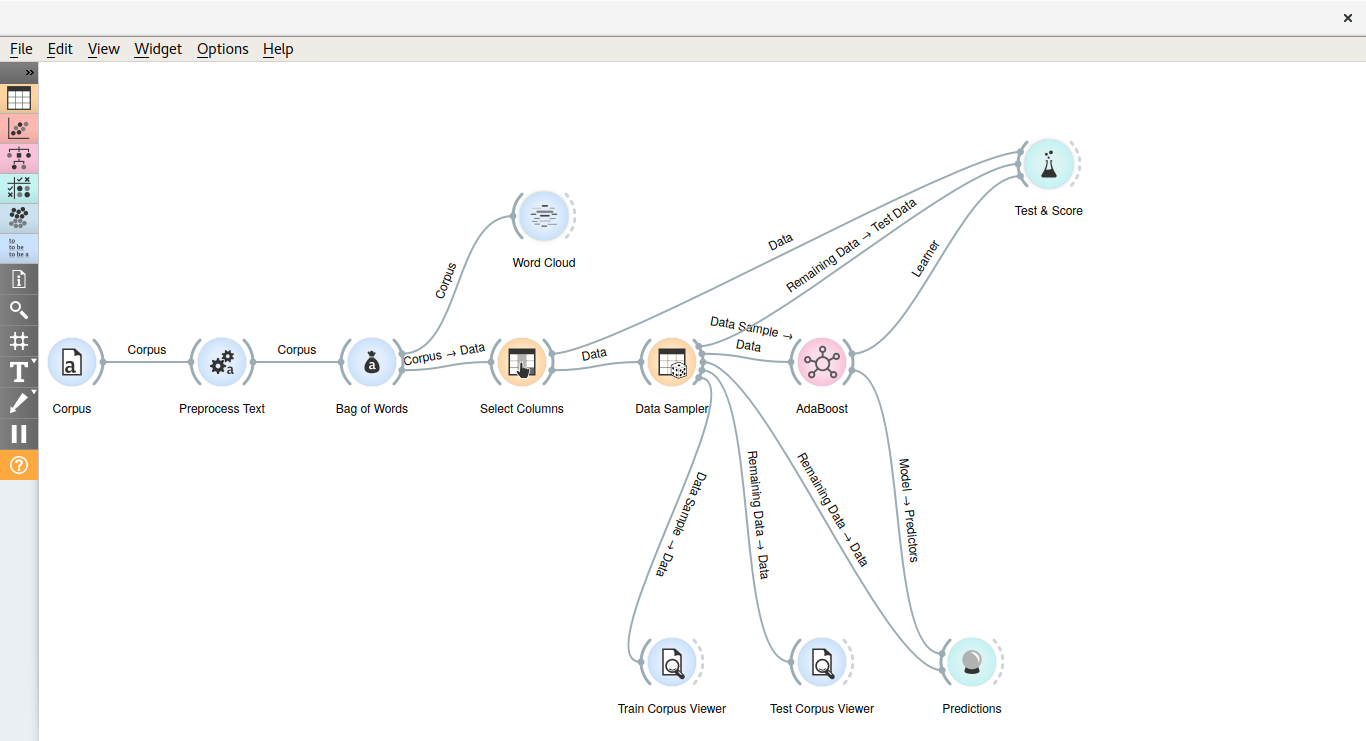
\includegraphics[scale=0.30]{figuras/orange_canvas.png}
\end{center}
\caption{Interface gráfica \textit{Orange Canvas}}
\label{fig:orange_canvas}
\end{figure}

% Este objetivo foi relevante para nosso estudo porque sabemos que as condições de
